% !TeX program = LuaLaTeX
\documentclass[a4paper,oneside]{book}
\usepackage{comment} % enables the use of multi-line comments (\ifx \fi) 
\usepackage{lipsum} %This package just generates Lorem Ipsum filler text. 
\usepackage[left=0.5in,right=2in]{geometry}
\usepackage{amsmath}
\usepackage{amssymb,amsthm}  % assumes amsmath package installed
\newtheorem{theorem}{Theorem}
\newtheorem{corollary}{Corollary}
\usepackage{graphicx}
\usepackage{tikz}
\usetikzlibrary{arrows}
\usepackage{verbatim}
\usepackage{float}
\usepackage{tikz}
    \usetikzlibrary{shapes,arrows}
    \usetikzlibrary{arrows,calc,positioning}

    \tikzset{
        block/.style = {draw, rectangle,
                        minimum height=1cm,
                        minimum width=1.5cm},
        input/.style = {coordinate,node distance=1cm},
        output/.style = {coordinate,node distance=4cm},
        arrow/.style={draw, -latex,node distance=2cm},
        pinstyle/.style = {pin edge={latex-, black,node distance=2cm}},
        sum/.style = {draw, circle, node distance=1cm},
    }
\usepackage{xcolor}
\usepackage{mdframed}
\usepackage[shortlabels]{enumitem}
\usepackage{indentfirst}
\usepackage{hyperref}
\usepackage{mhchem}
\usepackage{titlesec}
\usepackage{fontspec}
\usepackage{titlesec, blindtext, color}
\usepackage{tcolorbox}
\usepackage{caption}
\usepackage{sidenotes} 
\usepackage{esdiff}
\renewcommand{\thesubsection}{\thesection.\alph{subsection}}
\usepackage{esvect}
\usepackage{pdfpages}

\renewcommand{\qed}{\quad\qedsymbol}
\setlength\parindent{0pt}

\usepackage{listings}


\definecolor{dkgreen}{rgb}{0,0.6,0}
\definecolor{gray}{rgb}{0.5,0.5,0.5}
\definecolor{mauve}{rgb}{0.58,0,0.82}

\lstset{frame=tb,
  language=Python,
  aboveskip=3mm,
  belowskip=3mm,
  showstringspaces=false,
  columns=flexible,
  basicstyle={\small\ttfamily},
  numbers=none,
  numberstyle=\tiny\color{gray},
  keywordstyle=\color{blue},
  commentstyle=\color{dkgreen},
  stringstyle=\color{mauve},
  breaklines=true,
  breakatwhitespace=true,
  tabsize=3
}




\begin{document}
\begin{titlepage}
    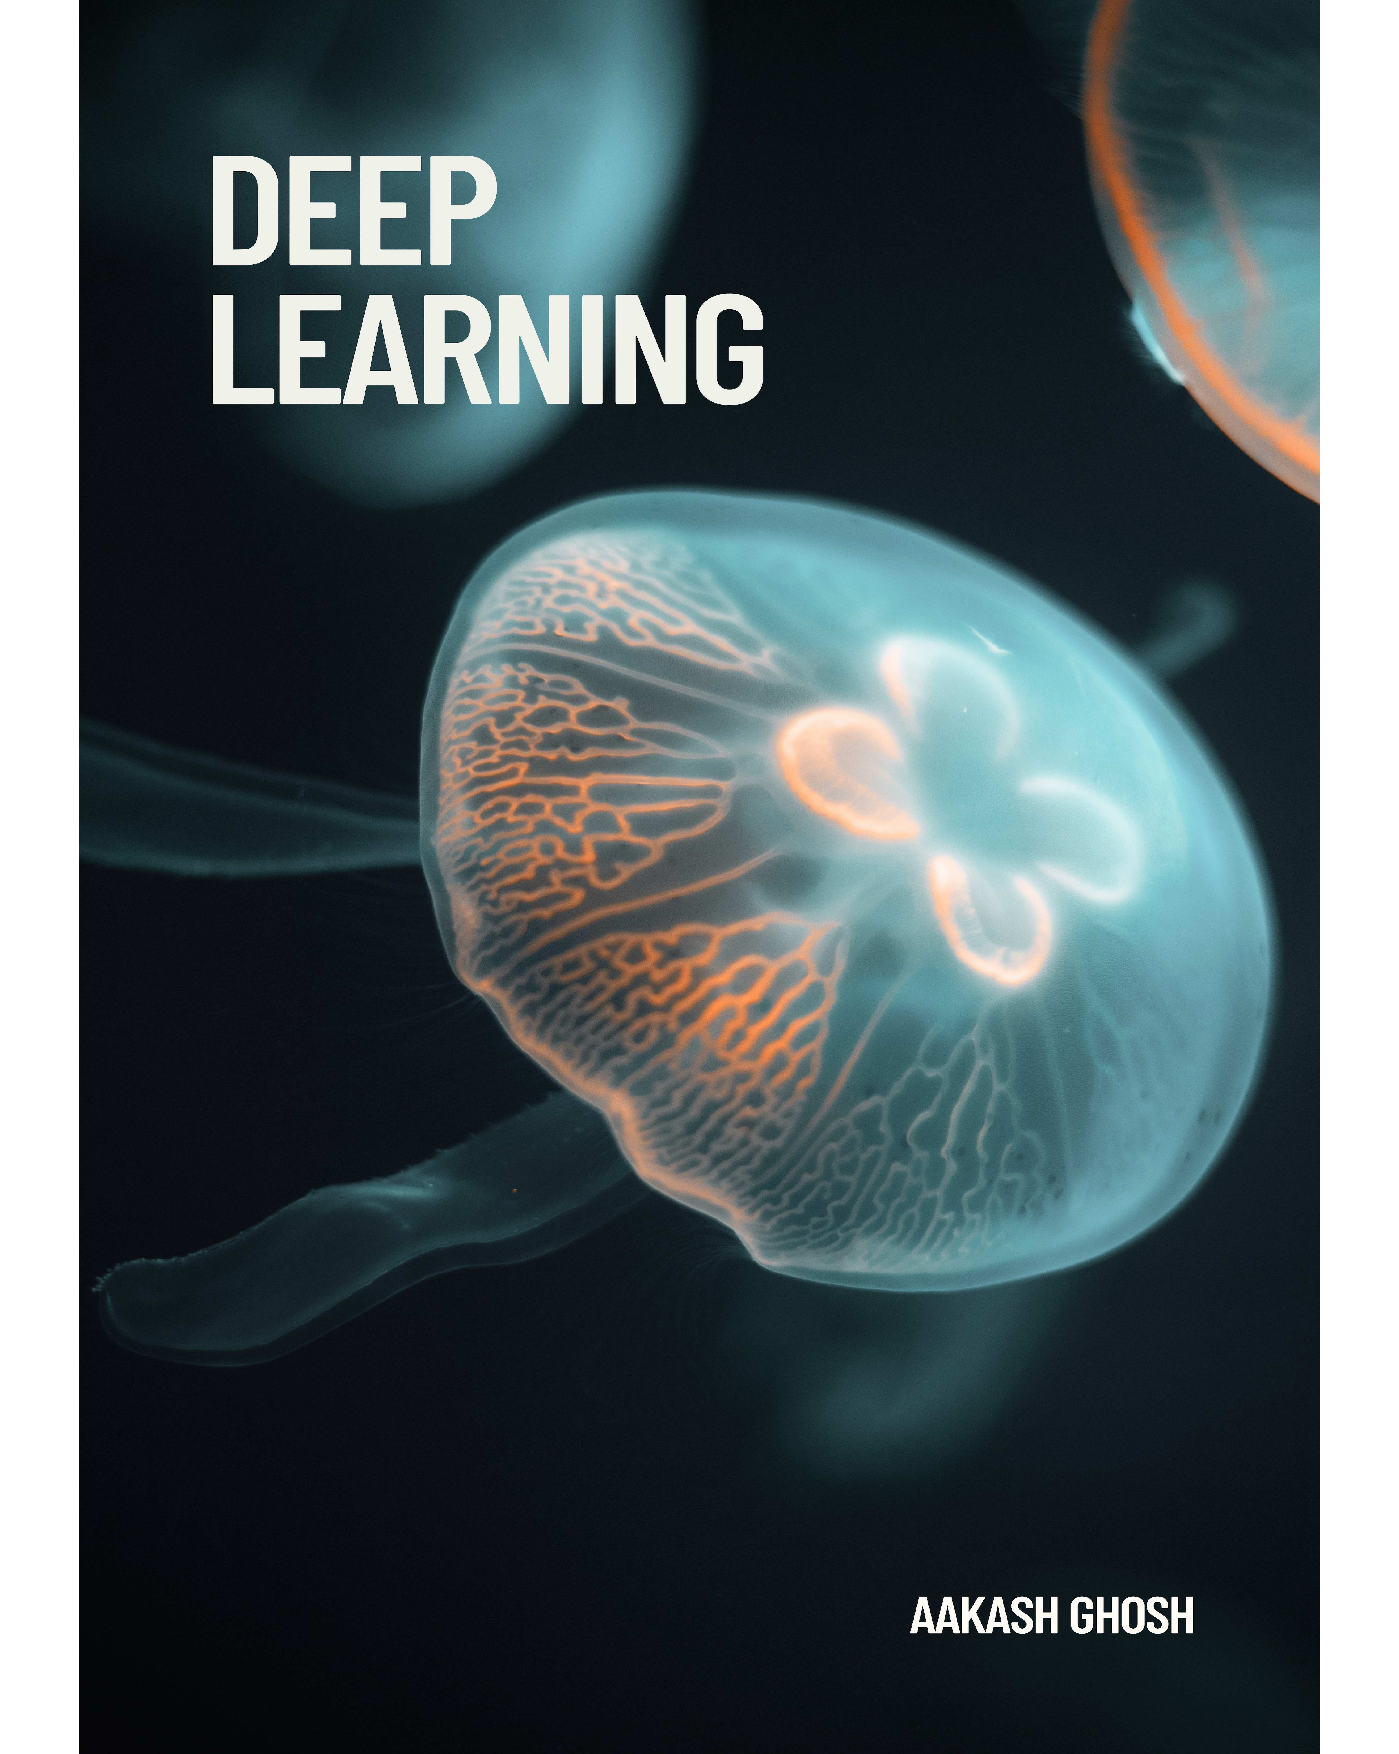
\includepdf[fitpaper]{images/cover}
\end{titlepage}
\clearpage
\newpage
\newpage
%\setmainfont{KITTY CAT}
%\setmainfont{Meows}

\tableofcontents

\newgeometry{top=5mm, bottom=10mm,left=0.5in,right=0.5in}

\part{Theory of Deep Learning}

\restoregeometry


\chapter{Deep Learning}
    \begin{marginfigure}%
        %
\includegraphics[width=2.4\marginparwidth]{graphics/(40).png}
    \end{marginfigure}%
\section{Traditional Machine Learning}
    Traditionally, solving a problem by machine 








\newgeometry{top=5mm, bottom=10mm,left=0.5in,right=0.5in}

\part{Natural Language Processing for Deep Learning}

\restoregeometry


\chapter{Natural Language Processing}

\section{Introduction}

    Language arose about $100,000-1,000,000$ years ago. As it turned out, the biggest power was not fangs and poison but communication. And it was language and writing that took us from Bronze Age to modern science. As far as AI is concerned we have made large progress. Machine translation are readable (even if all the nuances are not conveyed). The single biggest development was of course GPT3. One of the key feature was that it was a universal model: we no longer need different classifier/neural network to o different task, one universal model was enough.

\section{Laguage modelling}

    A word is the verbal/written representation of idea. Traditionally, a computer understands a word by using a dictionary and looking up synonyms(word with similar meaning), hypernyms(expression of belonging to a more general category), hyponyms(expression of belonging to more specific subclass). A minimal example implemented in NLTK is shown below. Some arrays are truncated for brevity.
    \begin{lstlisting}
        >>> from nltk.corpus import wordnet as wn
        >>> wn.synonyms('car')
        [['auto', 'automobile', 'machine', 'motorcar'], ['railcar', 'railroad_car', 'railway_car'], ['gondola'], ['elevator_car'], ['cable_car']]
        >>> wn.synsets('car')[:2]
        [Synset('car.n.01'), Synset('car.n.02')]
        >>> wn.synset('car.n.01').definition()
        'a motor vehicle with four wheels; usually propelled by an internal combustion engine'
        >>> wn.synset('car.n.01').examples()
        ['he needs a car to get to work']
        >>> wn.synset('car.n.01').hypernyms()
        [Synset('motor_vehicle.n.01')]
        >>> wn.synset('dog.n.01').hypernyms()    
        [Synset('canine.n.02'), Synset('domestic_animal.n.01')]
        >>> wn.synset('car.n.01').hyponyms()[:5]
        [Synset('ambulance.n.01'), Synset('beach_wagon.n.01'), Synset('bus.n.04'), Synset('cab.n.03'), Synset('compact.n.03')]
    \end{lstlisting}
    But this is not a very robust solution: it should be trivial to note that meaning of words are often dependent on context and nuances are not conveyed(Ex: "crimson" is a synonym of "red" but "the color of an apple is crimson" is a weird sounding sentence).  Moreover, language is ever-changing and keeping up to date is hard. 
    \begin{marginfigure}%
        
    \end{marginfigure}%
    In traditional bag of words approach, words are given a one hot vector representation. For example:
    \begin{align*}
        \text{"hotel"}=[0,0,0,0,0,1,0,0,0]\\
        \text{"motel"}=[0,0,0,0,0,0,0,1,0]
    \end{align*}
    But this approach has its own limitations:
    \begin{enumerate}
        \item Vector size increase with increase in vocabulary
        \item We understand that the words above are similar, but that similarity is not reflected in such one-hot encoding.
    \end{enumerate}





























\end{document}





